\begin{figure}
  \centering
  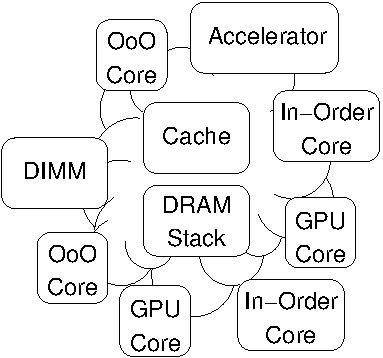
\includegraphics[width=2in]{fig/arch}
  \caption{Thanks to the flexibility of the simulation infrastructure, the system architecture of \name can remain defined only as a set of components. Where these should located and in what topology they should be connected is the topic of future research.}
  \label{fig:arch}
\end{figure}

Figure~\ref{fig:arch} illustrates the architecture of a \name system; notable for its lack of structure.
It is not yet clear at this early point in the development of PNM architectures exactly what their high-level structure should be.
With a flexible simulation infrastructure we will be able to explore a variety of possible system-level architectures, including combinations of:
\begin{itemize}
  \item Networks-on-chip.
  \item In-package integration with DRAM stacks.
  \item 3D-stacked integration with DRAM stacks.
\end{itemize}

Micron's Hybrid Memory Cube (HMC) \cite{hmc} is one of the most promising emerging stacked DRAM technologies.
FPGA products with HMC interfaces have recently been announced. \cite{hmcfpga}
This combination of FPGA and stacked memory is an attractive target for prototype near-memory architectures.
Prototypes built in such a manner would hardly qualify as having PNM architectures, but their designs would share much more with PNM architectures than they would with DDR-based systems.
